%%%%%%%%%%%%%%%%%%%%%%%%%%%%%%%%%%%%%%%%%
% Design based on a template by Roberto and following the format of
% the xmipp tutorials. In turn, they seem to be based on a template
% from http://www.latextemplates.com
%%%%%%%%%%%%%%%%%%%%%%%%%%%%%%%%%%%%%%%%%

%----------------------------------------------------------------------------------------
%	PACKAGES AND OTHER DOCUMENT CONFIGURATIONS
%----------------------------------------------------------------------------------------

\documentclass[12pt]{article} % Default font size is 12pt, it can be changed here
\usepackage[english]{babel}
\usepackage[utf8]{inputenc}
\usepackage{listings} % To include source code
\usepackage{caption}
\usepackage{geometry} % Required to change the page size to A4
%\geometry{a4paper} % Set the page size to be A4 as opposed to the default US Letter
\usepackage{framed}
\usepackage{url}
\usepackage{graphicx} % Required for including pictures
\usepackage{natbib}
\usepackage{float} % Allows putting an [H] in \begin{figure} to specify the exact location of the figure
\usepackage{hyperref}
\usepackage{menukeys}
\usepackage{array}
\usepackage{fancyhdr}
\usepackage{marvosym}%smileys\Smiley{} \Frowny{}
\usepackage{etoolbox}
\usepackage{listings}
\usepackage{makecell}
\usepackage{marginnote}
\usepackage{soul}
% \usepackage[T1]{fontenc}
%\usepackage{color}
%\sethlcolor{lime}
\sethlcolor{yellow}
%\sethlcolor{orange}

%\renewcommand{\hl}[1]{#1}
%pdflatex -jobname=students '\def\student{}\input{main}'
%pdflatex -jobname=teachers '\def\teachers{}\input{main}'
%  \ifdef{\teachers}
%  {Content for teachers}
%  {Content for students}
\newcommand{\ttt}[1]{\texttt{#1}}
\newcommand{\iii}[1]{\textit{#1}}
\newcommand{\ra}{$\rightarrow$}
\pagestyle{fancy}
\fancyhf{}
\fancyhead[RO]{{Model Building}}
\fancyhead[LO]{Scipion}
%\fancyhead[RO]{{\leftmark}}
\fancyfoot[RO]{\thepage}

\linespread{1.2} % Line spacing

%\setlength\parindent{0pt} % Uncomment to remove all indentation from paragraphs

\newcommand{\scipion}{\textsc{Scipion} }
\newenvironment{command}{\tt\begin{quote}}{\end{quote}}
\newcommand{\comm}[1]{\texttt{#1}}

\newcommand{\imgfig}[3]{\begin{figure}[H]\centering \
\includegraphics[scale=#2]{images/#1} \caption{#3} \end{figure}}

\newcommand{\proto}[1]{\textit{\textbf{#1}}}
\newcommand{\popt}[1]{\textit{#1}}
\newcommand{\pval}[1]{\texttt{#1}}

\newcommand\tstrut{\rule{0pt}{2.4ex}}
\newcommand\bstrut{\rule[-1.0ex]{0pt}{0pt}}

\def \humanAdenoMap {7034}%5172

\begin{document}

%----------------------------------------------------------------------------------------
%	TITLE PAGE
%----------------------------------------------------------------------------------------

\begin{titlepage}

% New command for horizontal lines. Change thickness here.
\newcommand{\HRule}{\rule{\linewidth}{0.5mm}}

\center % Center everything on the page


\includegraphics{images/scipion_logo.png}

{\large Scipion Tutorial Series}\\[1.0cm]

\textsc{\LARGE National Center for Biotechnology}\\[0.5cm]
\textsc{\Large Biocomputing Unit}\\[0.15cm]

\HRule\\[0.4cm]
{ \huge \bfseries Model Building}\\ % Title of your document
\HRule \\[0.5cm]
%{\large \today}\\[3cm] % Date, change the \today to a set date if you want to be precise
\begin{center}
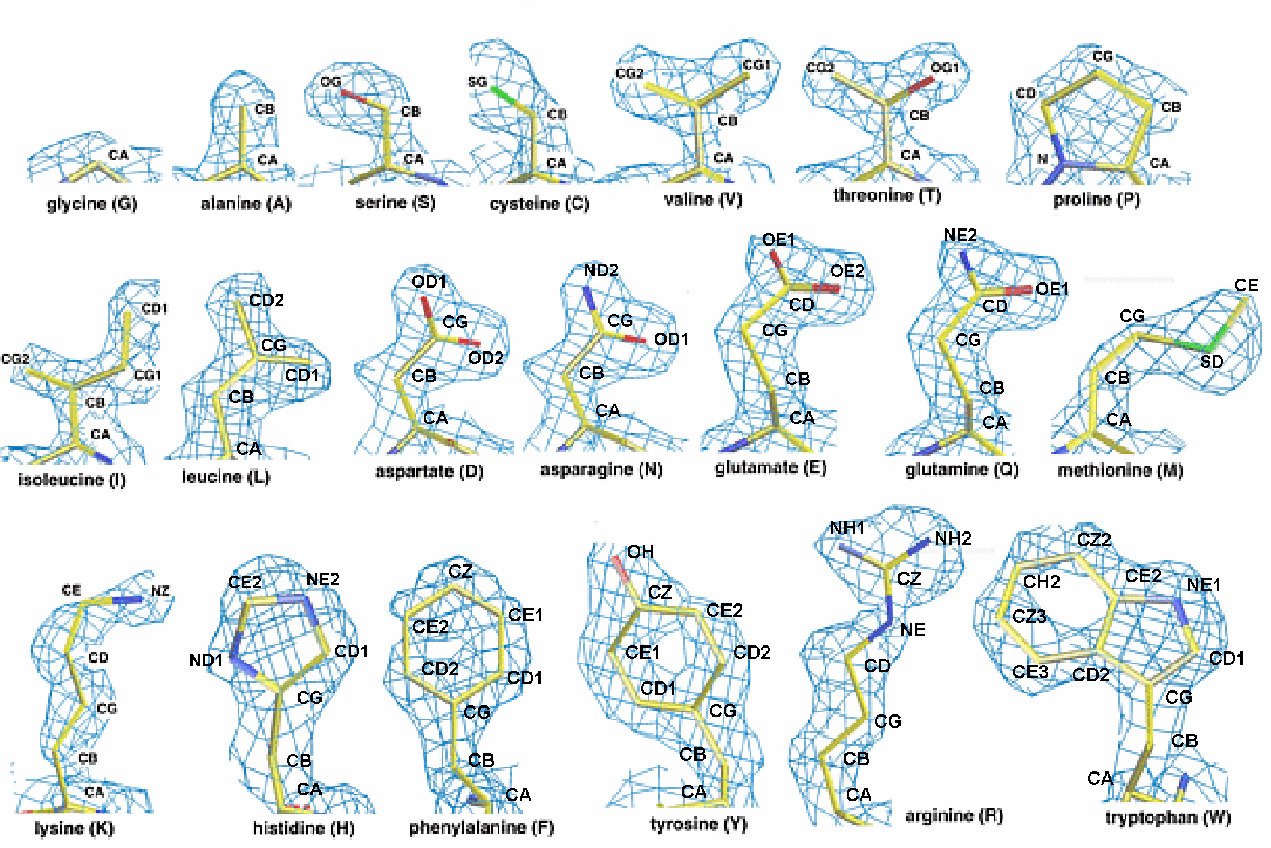
\includegraphics[width=0.70\textwidth]{{images/aadensity}.png}\\
Density for amino acid side chains from an experimental electron density map at 1.5 \AA~resolution (http://people.mbi.ucla.edu/sawaya/m230d/Modelbuilding/modelbuilding.html)\end{center}

%\vfill % Fill the rest of the page with whitespace
%\begin{minipage}{0.4\textwidth}
\begin{flushright}
 \large
%\emph{Author:}\\
  \textsc{Roberto Marabini} % Your name
\end{flushright}
%\end{minipage}

\end{titlepage}


%----------------------------------------------------------------------------------------
%	OBJETIVOS
%----------------------------------------------------------------------------------------


\subsection*{Intended audience}
The recent rapid development of single-particle electron cryo-microscopy (cryo-EM) now allows structures to be solved by this method at resolutions close to 3\AA.  This tutorial provides an introduction to model building for cryo-RM data. %tomography in  electron microscopy with special emphasis in basic image processing. The tutorial requires matlab but does not assume any programing skills. 


\subsection*{We'd like to hear from you}

We have tested and verified the different steps described in this demo
to the best of our knowledge, but since our programs are in continuous
development you may find inaccuracies and errors in this text. Please
let us know about any errors, as well as your suggestions for
future editions, by writing to
\href{mailto:scipion@cnb.csic.es}{scipion@cnb.csic.es}.


\subsection*{Requirements}

This tutorial requires, in addition to $Scipion$,  the \textit{CCP4 suite} including $refmac$ and $coot$ as well as $USCF Chimera$. Basic knowledge of USCF Chimera and $Scipion$ is assumed. Warning: all versions of $refmac$ are not suitable for EM data. 

%\subsection*{Acknowledges}
%This tutorial uses material created at the Computer Vision Laboratory, Linkoping University, Sweden


\newpage


%----------------------------------------------------------------------------------------
%	TABLE OF CONTENTS
%----------------------------------------------------------------------------------------

\tableofcontents % Include a table of contents

\newpage % Begins on a new page instead of on the same page as the table of contents


\section{Introduction}
Single-particle electron cryo-microscopy (cryo-EM) is currently undergoing a technical revolution that  has allowed the structures of macromolecules to be solved at near-atomic resolution. That is, the density map is sufficiently resolved to build an atomic model. At resolutions of \hl{4.5\AA~ the C-$\alpha$ backbone} of the protein can be built based on the map alone, and at resolutions better than \hl{4.0\AA~some amino-acid side chains can be traced}. In the following we describe some tools to refine the models using constrains derived from prior knowledge as well as to validate the results. \hl{This tutorial is not an exhaustive description of the many approaches} and programs available for these tasks but it will introduce the field by presenting a full example.

 \begin{figure}[H]
 \centering
 \includegraphics[width=0.5\textwidth]
 {{charts/workFlow}.pdf}
 \caption{ Model Building Workflow}
 \label{fig:model_build_workflow}
 \end{figure}

\section{The Data}
The \hl{problem} that we  will  solve in this tutorial is,  given a \hl{3D map of human adenovirus} type 5 (EMD\_\humanAdenoMap)  at 3.2\AA~resolution and the sequence of its different proteins, how to build an atomic model. We will use as \hl{reference} the atomic model (PDBe-3zif) computed for the \hl{\textit{Bovine adenovirus 3}} (EMD-2273). In particular we will \hl{focus in the penton} protein. Pentons are the main proteins responsible of the  12 vertices of the virus capsid and contain the  \hl{arg-gly-asp motif} ($RGD$)  that is bounded by the cellular integrins and trigger endocytosis. \textit{A priory}, it is expected that the  $RGD$ loop (between aminoacids 300-370 approx.) will show the greater variability.

 \begin{figure}[H]
 \centering
 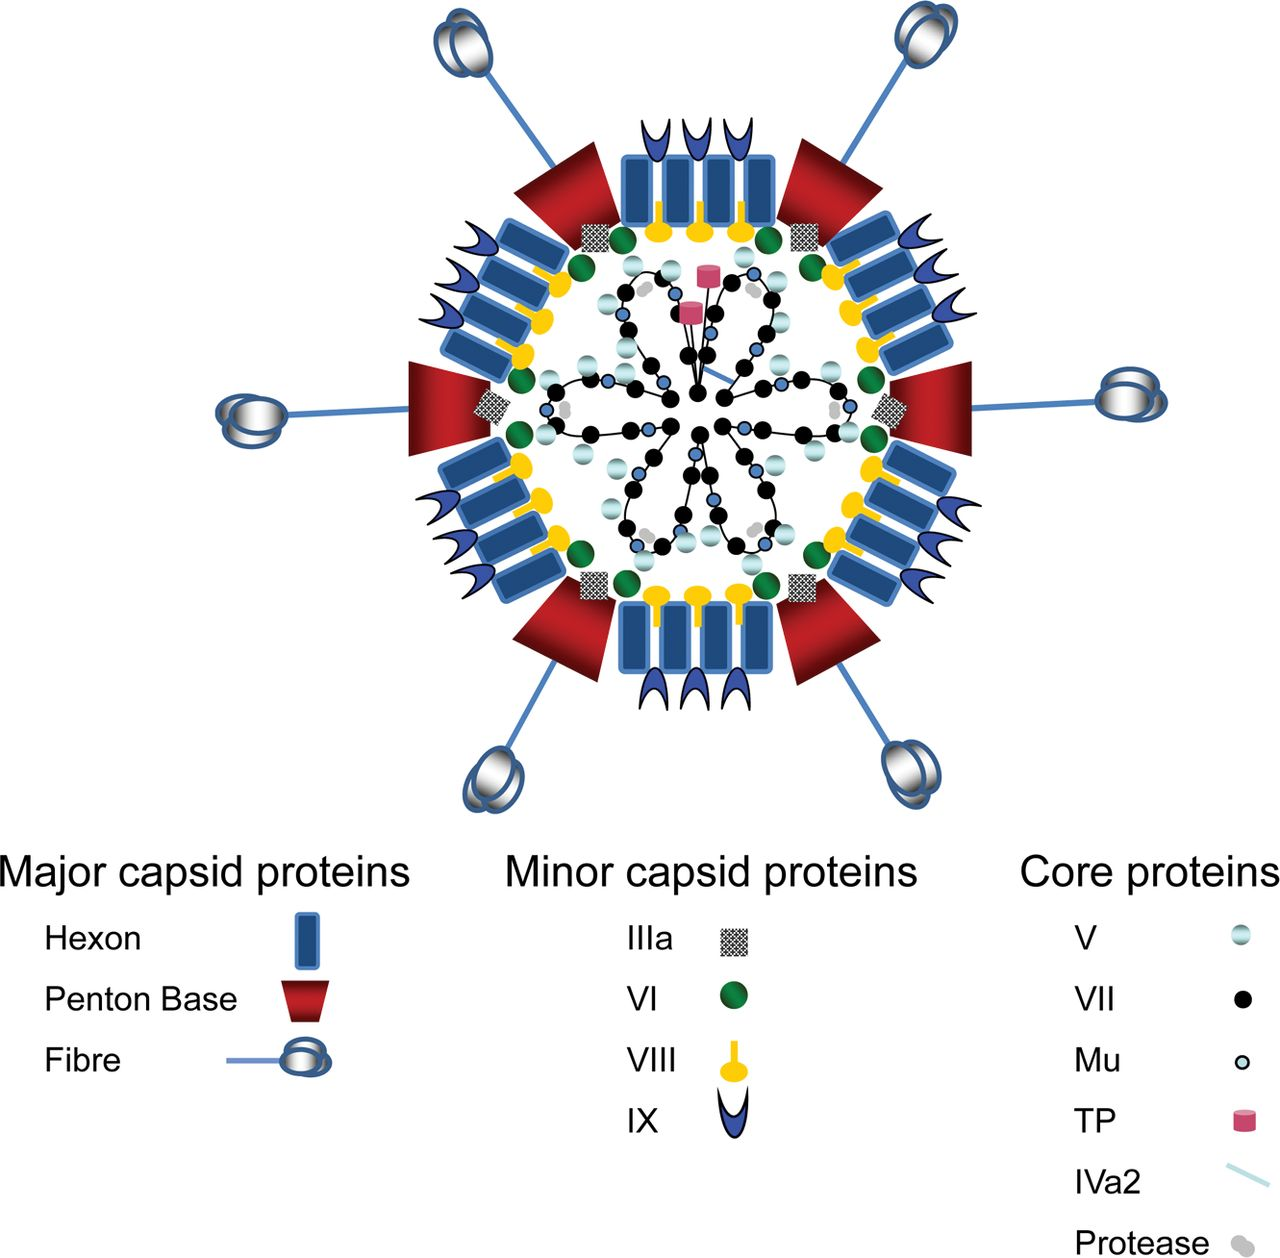
\includegraphics[width=0.7\textwidth]
 {{images/adeno_scheme}.png}
 \caption{ A schematic representation of the 13 structural proteins associated with the Adenovirus capsid. Image from Hall \textit{et al}. DOI: 10.1042/BJ20100766}
 \label{fig:adeno_scheme}
 \end{figure} 

 In order to follow this tutorial \hl{we will need}:
\begin{itemize}
 \item \textit{Bovine adenovirus 3} atomic model.
 \item human adenovirus type 5 sequence.
 \item human adenovirus type 5 3D map.
\end{itemize}

\reversemarginpar
\marginnote{\hl{Download data. Rsync}}[1cm]

The human adenovirus type 5 3D map may be downloaded from \url{http://www.ebi.ac.uk/pdbe/entry/emdb/EMD\_\humanAdenoMap}. Please, download the 3D map and call it $emd\_\humanAdenoMap.map$. The  penton sequence is available at \url{http://www.ebi.ac.uk/pdbe/entry/pdb/3iyn/protein/2}. Copy the sequence and save it in a file called \textit{\humanAdenoMap\_p.fasta}. Finally, let us download our reference PDB file (\url{http://www.ebi.ac.uk/pdbe/entry/pdb/3zif}, -\textit{Bovine adenovirus 3}-) an name it  \textit{pdb3zif.ent}. (An alternative source of data is \url{https://sites.google.com/site/scipionmb/home}.) \textit{pdb3zif.ent} contains a full asymmetric unit cell but we are going to work only with the penton so we need to edit it and save a single chain. 

\marginnote{\hl{Extract pentom. Chimera}}[1cm]
\begin{itemize}
 \item Open the file with chimera (\texttt{chimera pdb3zif.ent})
 \item In \texttt{favorites} select \texttt{model panel} and \texttt{command line}
 \item In \texttt{command line} type \texttt{split \#0} (18 entries will appear in the \texttt{control panel})
 \item Choose the entry identified with the letter $M$ (model $0.13$) 
 \item In \texttt{control panel} select \texttt{write PDB} and save the chain as $3zif\_p.pdb$ (do not forget to check the  \iii{save relative to model} option.) 
\end{itemize}

In order to check that the penton has been properly extracted

\begin{itemize}
 \item Open the file with chimera (\texttt{chimera 3zif\_p.pdb}). (Double check that chimera was only 
 loaded the penton, if the whole virus is loaded this operation may take a long while).
 \item In \texttt{favorites} select \texttt{command line}
 \item In \texttt{command line} type \texttt{sym \#0} 
 \item You should see the 12 vertices of the icosahedron. 
 \item If you type in the command line \texttt{shape icosahedron radius 400 orientation  222r} a icosahedron will be painted.
\end{itemize}

Now, you are ready to go \Smiley{}.


\section{Structure Prediction by homology}
\marginnote{\hl{swissmodel}}[1cm]
When predicting by homology a structure is constructed by aligning a target protein sequence with known template structures. The protein sequence can be obtained from many sources, for example NCBI or UniProt. The quality of a structure depends upon the similarity between the target sequence and the database sharing highest similarity is aligned. 

A first approach could be to connect to any of the available on-line predictors as \url{https://swissmodel.expasy.org/} and follow the instructions (\textit{start modeling} $\rightarrow$  \textit{search for templates} $\rightarrow$ \textit{Select reference} $\rightarrow$\textit{build model}). An exhaustive list of web sites is available at \url{http://molbiol-tools.ca/Protein_tertiary_structure.htm}. Since we are  using a sequence already traced it is possible to get a perfect solution. In order to be closed to a realistic case select as reference structure a template with around 80\% of similarity and lunch the predictor. It is difficult to  estimate the total processing time since depend heavily on the site workload but 4 hours is a realistic guess. 

\marginnote{\hl{chimera}}[1cm]
In the mean time let us play a little bit with $chimera$. A first step in homology modeling is the identification of the best template structure using, in many cases,  pairwise sequence alignments obtained with FASTA and BLAST. In general, the user may choose between the found templates but cannot \hl{supply her own template} structure (if the structure is not in a public data base this is an important drawback). Fortunately, Chimera is able to perform structure modeling starting from a given pdb template.

\begin{itemize}
 \item open chimera.
 \item load $3zip\_p.pdb$.
 \item select Tools $\rightarrow$ sequence $\rightarrow$ sequence.
 \item In sequence window, Edit $\rightarrow$ Add sequence $\rightarrow$ paste target sequence (\textit{\humanAdenoMap\_p.fasta}) and press OK.
 \item In sequence window, Structure $\rightarrow$ Modeller (homology) (run via web service- \hl{you will need to apply for a password}).
 \item When finished click \texttt{quit}, 5 models will appear. Choose the one you like best. Save it as \textit{first\_guess\_p.pdb}, do not forget to select \textit{save relative to model}. (In chimera main window, lower left corner you may see the status of your job, allow 20 minutes for this step. The result of this step is available at \hl{\texttt{homologe\_prediction.py}})
 %\item In chimera, for my taste, ribons are too thin, if you want to make the ribbons thicker type \texttt{ribscale thick}  
\end{itemize}

\marginnote{\hl{wait 1}}[0cm]
\textcolor{gray}{While waiting coot intro}

\marginnote{\hl{wait 2}}[0cm]
\textcolor{gray}{While waiting jump to molprobity and check saccharomyces cerevisiae triosephosphate isomerase with 3ypi (2.8\AA-1991), 1ypi(1.9\AA-1990) and 1ney(1.2\AA-2003)}

\marginnote{\hl{comment}}[1cm]
As you can see there are two zones that are present in the human but not in the bovine Adenovirus.
Please write down the first and last amino-acids of these zones.\\
first\_aa1 $\rule{1cm}{0.15mm}$, last\_aa1 $\rule{1cm}{0.15mm}$\\
first\_aa2 $\rule{1cm}{0.15mm}$, last\_aa2 $\rule{1cm}{0.15mm}$\\
Why do you think the first zone is not present in the bovine Adenovirus? and the second zone?

 \begin{figure}[H]
 \centering
 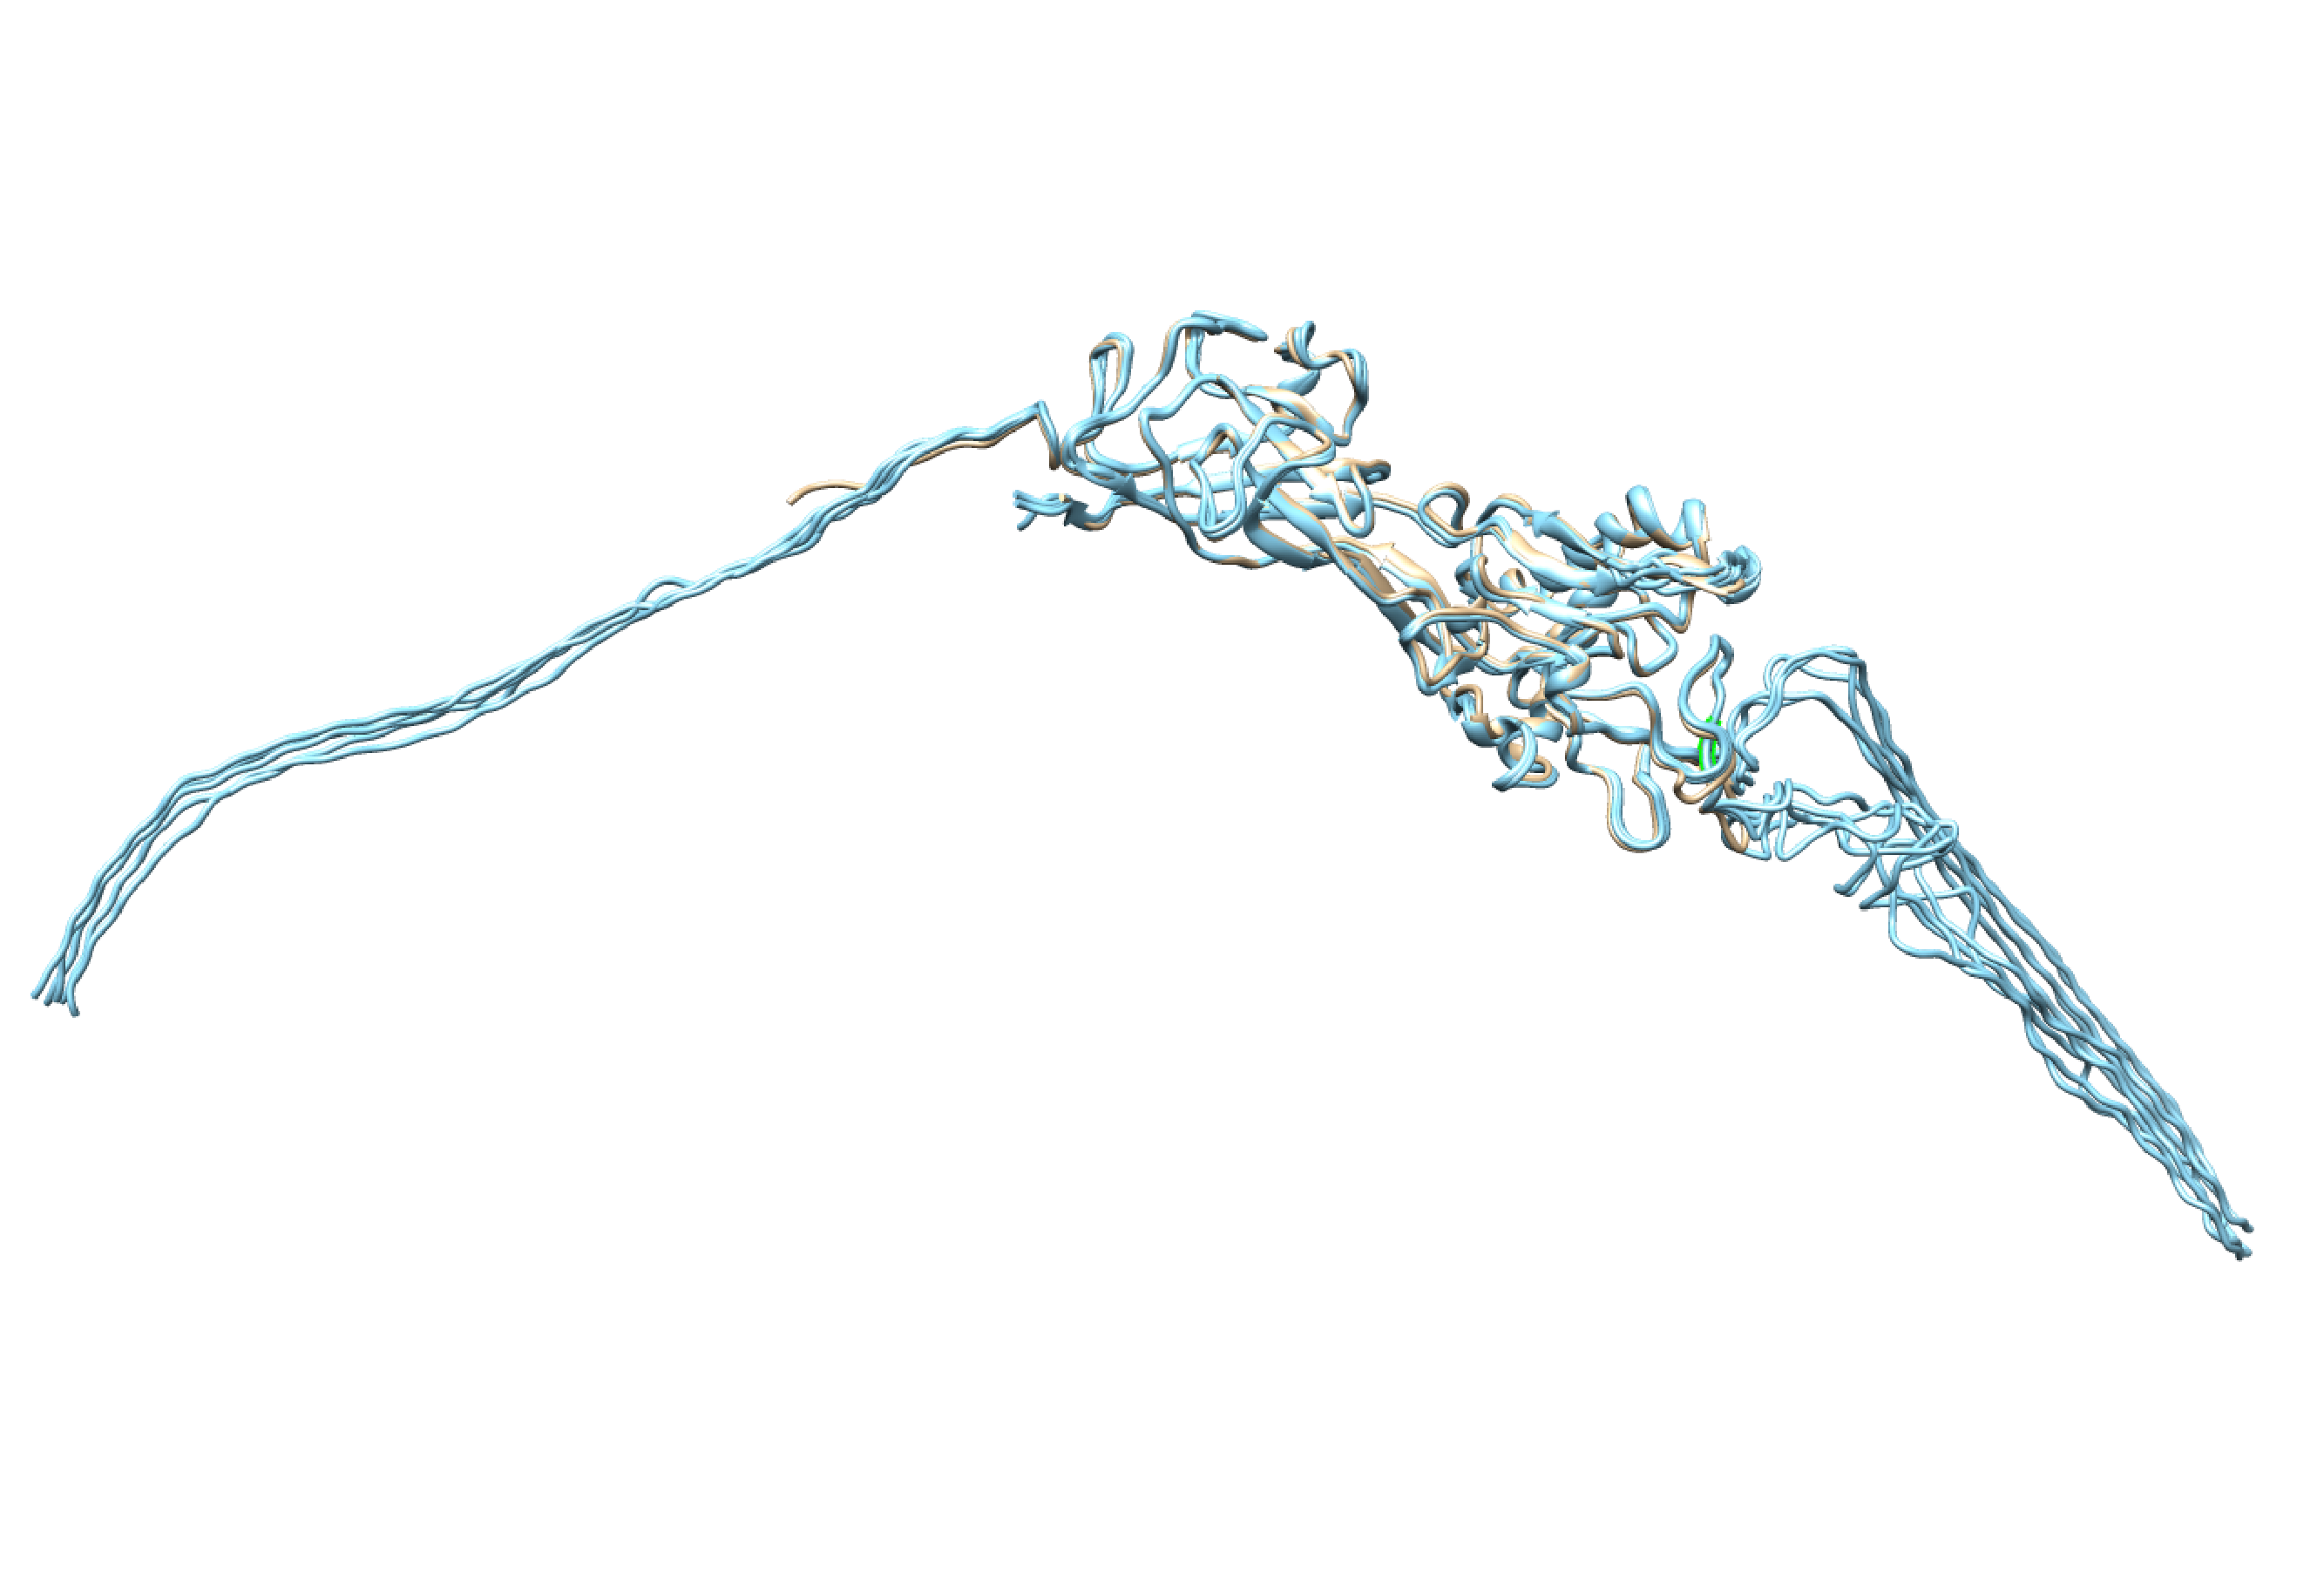
\includegraphics[width=0.7\textwidth]
 {{images/reference_targets}.png}
 \caption{Result of executing in chimera the Structure Modeler tool}
 \label{fig:chimeramodelbuild}
 \end{figure} 
% Two receptor: car, integrin in the cell
% fiber joins car (movile), when arive close integrine RGD join integrin
% car movie fiber goes away
% cell identifies virus as something interesting to be incorporated
 
%chimera password MODELIRANJE 
 
%1-38, ask for clereave
%293-373
\subsection{Secondary prediction}
   
   Before going ahead let us run a secondary structure prediction. Hopefully the unknown regions will show some structure that may help us to trace the pentom chain. Connect to \url{http://bioinf.cs.ucl.ac.uk/psipred/} follow the instructions (that is, paste sequence at \textit{Input Sequence}, provide a \textit{Short identifier for submission}, click \textit{predict}) and save the 
   results (Download $\rightarrow$PDF version of the PSIPRED diagram) in a file called \textit{secondary\_prediction.pdf}. \hl{Compare this secondary prediction with the results provided by chimera}.

\section{Preparing the Data}
\marginnote{\hl{preprocess}}[1cm]
   We are almost ready to start tracing our chain but before we can start we need to: 
   (1) check that the 3D map file format and conventions are correct (I have never seem a reconstruction algorithm that satisfies this constrains)
   (2) put the ``guess structure'' (file \textit{first\_guess\_p.pdb}) in the same system of coordinates than the 3D map (\textit{emd\_\humanAdenoMap.map}) so that the software we are going to use for model building has a fair starting point.
   \subsection{Import Data to Scipion}
   \begin{itemize}
    \item Let us import the problem 3D map (\textit{emd\_\humanAdenoMap.map}) and PDB file (\textit{first\_guess\_p.pdb}). Open scipion and import the map  (\ttt{import volume}, samplingrate= 0.85) and the PDB file (\ttt{import PDB})
    \item Using the Analyze button double-check that both objects look OK. Visualize the 3Dmap using chimera, if chimera shows a single plane  click (in \textit{Volume Viewer}) \textit{All}, in \textit{style} select surface and increase the step to 4 (see Fig. \ref{fig:emd_\humanAdenoMap_view}). (The volume will look nicer if you 
    color it by radius. Select \ttt{volume}$\rightarrow$\ttt{surface color}, then click \ttt{by radius} and finally press \ttt{color}.
    \end{itemize}
    
   \subsection{Extract a unit cell}
    
%    \item execute the program \texttt{showheader.py  emd\_\humanAdenoMap.map} check that the header looks OK. If this is not the case fix it.\\ Exercise: In particular check that the sampling rate is OK, get data from experimental metadata (xml) in $EMD-\humanAdenoMap$ entry $samplingRate= \frac{samplingSize}{Magnification}$.
%\marginnote{\hl{careful}}[2cm]
    
    A virus is a very large volume with high symmetry. For today's task we only need a small portion of the 3D map. We are going to extract the non redundant part of the
    virus using the protocol \ttt{unit cell}. As parameters use \textit{Symmetry}: I222, \textit{Inner Radius(px)}: 200, \textit{Outer Radius(px)}: 640 and \textit{expand factor}: 0.1. 
    

     
    \begin{figure}[H]
    \centering
    \includegraphics[width=0.75\textwidth]
    {{images/emd_\humanAdenoMap_view}.png}
    \caption{human Adenovirus view in chimera}
    \label{fig:emd_\humanAdenoMap_view}
    \end{figure} 

%\marginnote{\hl{resmap}}[2cm]
%    Finally, we may execute \texttt{resmap} to get an idea on the local resolution. (use Scipion, import the volume \textit{emd\_\humanAdenoMap\_win\_norm.map} and then execute the protocol \texttt{3D} $\rightarrow$ \texttt{Analysis} $\rightarrow$ \texttt{resmap - local resolution}) in order to estimate the resolution at the different volume areas. Areas with a resolution higher than 4\AA will be difficult to trace. In order to see the results click on \texttt{Analyze Results} $\rightarrow$ \texttt{Show Chimera Animation}. After the animation is finished select \texttt{Volume Viewer} $\rightarrow$ \texttt{Features} $\rightarrow$ \texttt{Planes} and  click on \texttt{All}. After that select you may place a colorbar by: \texttt{Main window} $\rightarrow$  \texttt{Volume} $\rightarrow$ \texttt{surface color} $\rightarrow$ options $\rightarrow$ \ttt{volume data} $\rightarrow$ \texttt{create color key}, then click in the main window and grab the mouse.
    
 %   \begin{figure}[H]
  %  \centering
  %  \includegraphics[width=0.75\textwidth]
  %  {{images/resmap}.png}
  %  \caption{resmap output. Check the disagreement between the given and the reported %resolution. May it be caused by low pass filtering?}
  %  \label{fig:resmap}
  %  \end{figure} 
    
\section{Fitting}
We are done with the preprocessing. Now we are going to fit \textit{first\_guess\_p.pdb} into the 3D map obtained using \ttt{extract unit cell}. 

\begin{itemize}
\item In Scipion select \ttt{chimera Rigid fit}, select as \textit{input volume} and \textit{PDB file to be refined} the volume produced by \ttt{extract unit cell} and the imported PDB file (in the text I will refer to this PDB structure as penton). Then press \ttt{Execute}

\item Unfortunately the PDB file and the 3D map do not fit because the bovine and human adenovirus have been reconstructed using different symmetry. We know the one used for
the 3D map (since we reconstructed it) but we ignore the one related with the penton.

\item Using \textit{Tools} $\rightarrow$ \textit{High-Order Structure} $\rightarrow$ \textit{Icosahedron surface} try to discover the symmetry related to the penton.

\item Apply the symmetry to the penton: \ttt{sym \#[modelNumber] group i,[symmetry]}. 59 symmetry related copies of the penton will be created.

\item Delete all penton copies that are outside the unitcell. Hover the mouse over the chain to get the model ID.

\item SAVE chimera SESSION NOW!!!!

\item Very gently try to fit manually the penton in the 3Dmap

\item refine using \textit{volume viewer} $\rightarrow$ \textit{Tools}
$\rightarrow$ \textit{fit in Map}. Just fill the right values in \textit{Fit} and \textit{in map} and press \ttt{Fit}.

\item In order to asses the fitting quality, in \textit{volume viewer} set the \textit{style} to \textit{mesh} and using \textit{Favories} $\rightarrow$ \textit{Side View} select a very narrow map slice.

\item Finally save the fitted PDB using the command \textit{scipionwrite model \#{pdbNumber} refmodel \#{3Dmap} saverefmodel 1}

\end{itemize}

 We are ready to start model building  \Smiley.

 \marginnote{\hl{do this later}}[0cm]
Exercise: Check in the 3Dmap nominal scale by playing with  \ttt{Volume Viewer} \ra \ttt{Fit in Map} \ra \ttt{Fit} while you modify the voxel size  \iii{number $<$enter$>$}. In order to use this method properly it is better to use something massive as the hexon and remove loops that cannot be traced.
 
\section{Refine Fitting}
 \marginnote{\hl{coot tutorial}}[1cm]
 
 After the rigid fitting it is time to refine the atomic model using the 3Dmap.
   \begin{itemize}
      \item start the protocol \ttt{coot refinement}. Select as \textit{input volume} and \textit{PDB to be refined} the output produced my the \textit{chimera fit} protocol.
      Then press \ttt{execute}.
      \item \ttt{edit} \ra \ttt{map} \ra \ttt{map parameters}. Set \iii{map radius = 30}.
      In \ttt{edit} \ra \ttt{general} \ra \ttt{Smooth recentering} set \textit{Number of steps}=5
   \end{itemize}
   
    \begin{figure}[H]
    \centering
    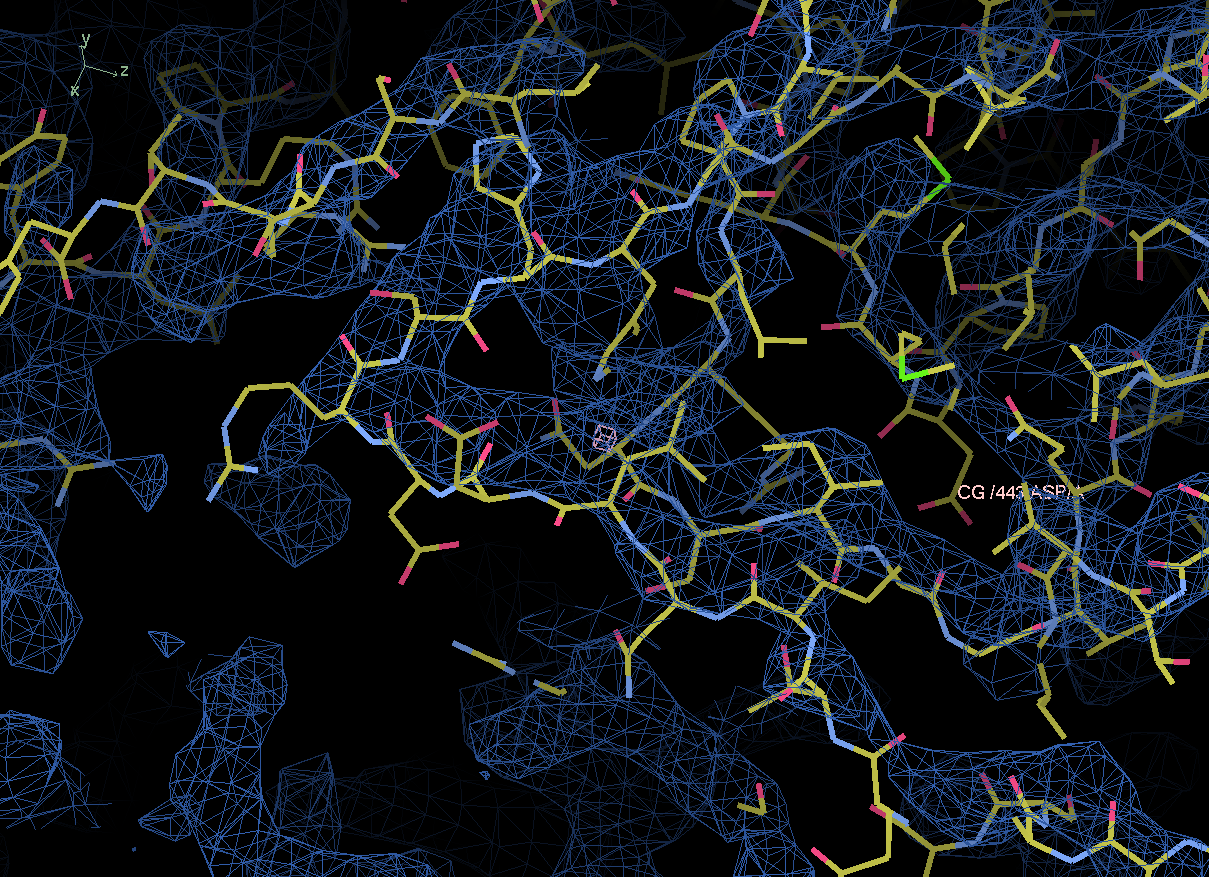
\includegraphics[width=0.75\textwidth]
    {{images/coot_simple}.png}
    \caption{Coot screen-shoot.}
    \label{fig:coot}
    \end{figure} 
    
\subsection{Interlude: Get comfortable with coot}

Play a little with your mouse using the following mouse actions that will rotate, shift, zoom and change clipping (thickness of the visualized slice).\\

\begin{tabular}{ l l }
  \hline
  Left-mouse Drag  & Rotate view\\\hline
  Ctrl Left-Mouse  & Drag Translates view\\\hline
  Shift Left-Mouse & Click Label Atom\\\hline
  Right-Mouse Drag & Zoom in and out\\\hline
  Ctrl Right-Mouse & \makecell[l]{Horizontal drag: Change clipping\\ 
                     Vertical drag: Translate along screen~Z~axis.}\\\hline
  Middle-mouse & Click Center on atom\\\hline
  Scroll-wheel & Forward Increase map contour level\\\hline
  Scroll-wheel & Backward Decrease map contour level\\\hline
\end{tabular}\\

Exercise: Look for an alpha helix with 5 loops.

\subsection{Some basic coot functions}

  \begin{tabular}{ l l }
  \hline
  Go to atom  & 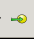
\includegraphics[width=1cm]{{images/coot_go_to_atom}.png} (F6)\\\hline
  Refine and regularization parameters & R/RC\\\hline
  Real Space Refine  & 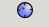
\includegraphics[width=1cm]{{images/real_space_refine}.png}\\\hline
  %Rigid body Fit & Click Label Atom\\\hline
  Rotate translate Zone & 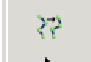
\includegraphics[width=1cm]{{images/rotate_translate_zone}.png}\\\hline
  Rotamers & 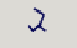
\includegraphics[width=1cm]{{images/rotamers}.png}\\\hline
  space & go next atom\\\hline
  shift space & go previous atom\\\hline
    
\end{tabular}\\  
  Exercise: go to atom 179, select alpha helix in $R/RC$ and \iii{real space refine} the helix.
  Exercise: continue tracing the chain another 20 aa., select no secondary structure in $R/RC$ and \iii{real space refine} the chain.
%\url{https://www.ccp4.ac.uk/schools/APS-2011/tutorials/coot/coot-chicago-june-2011-model-building+ncs.pdf}
\subsection{Change Chain IDs and Renumber Residues}
Sometimes is useful to be able to renumber residues and subtract subchains from a larger chain. These two functionalities are available through the \iii{Edit} menu. (\ttt{Edit} \ra \ttt{Change Chain ID}  and \ttt{Edit} \ra \ttt{Renumber Residues})

Exercice: go to the first atom, follow the chain till you find some density and rename this part of the chain that cannot be traced as x. Repeat the operation with the loop that start around aa. 300

Exercise: travel though the whole chain. If you see any evident large mismatch fix it. Do not worry to much, yet, about details o large disagreements.	 Save the resulting PDB file as coot\_pentom\_1.pdb. Save only the A chain, not the x. In order to delete the chain,
\begin{itemize}
 \item click on the red icon (\iii{Delete Item}) in the toolbar and select \iii{Delete zone}
 \item go to the first residue in the chain (in the Go to atom window), click on the residue
 \item similarly, go to the last one and click that
\end{itemize}
Coot should delete the chain (it will take a while if it is a large one)

\subsection{Other options to try}
 Extension $\rightarrow$ All Molecule $\rightarrow$ Fit Protein?\\
 Extension $\rightarrow$ modelling $\rightarrow$ residues with cis peptides bonds\\
%cis
%b-factor

\newpage
UP TO HHHHHHHHHHHHHHHHHHHHHHHHHHHHHHHHHHHHERE



\section{RefMac}
\marginnote{\hl{update script}}[1cm]
Model refinement is performed to maximize the agreement between the model and experimentally observed data and to minimize stereochemical violations. We have make some basic manual refinement let us see if this first guess is enough for a automatic refinement algorithm as Refmac. You would need the script refmac-EM.

Current version of the program uses automatic weighting. For many cases it works
sufficiently well. For low resolution you may want to
use very small weights -0.01 or even smaller (this is generally the case for EM data). For higher resolution this number may need to be as high as 10. You may need to run refinement with different
values to get it right. Check the logs for rms values -at the file end. If after refinement the \iii{rms bond lengths} are more than 0.02 then you may want to reduce weighting, if rms bond value is less than 0.01 then you may need to increase it. 

\begin{verbatim}
#example of rms values
 R factor 0.1876 (less than .3)
 Rms BondLength 0.0201 (about 0.02); (r.m.s. deviations from idealized bond lengths)
 Rms BondAngle 1.6554
 Rms ChirVolume 0.1063
\end{verbatim}


(Chiral volume of an atom that makes three bonds; the chiral volume is the volume of the 'unit-cell' (i.e. parallelepiped) whose axes are represented by these three bonds. The sign of the volume depend on the relative disposition of the three atoms).

NOTE: double check that the PDB file has a  CRYST card that agrees with the box size of the map
\begin{verbatim}
CRYST1  221.100  221.100  221.100  90.00  90.00  90.00 P 1   
\end{verbatim}


\section{Coot: validate}

\ttt{validate} \ra \ttt{Ramachandran plot}: Ramachandran diagram is a way to visualize energetically allowed regions for backbone dihedral angles $\psi$ against $\phi$ of amino acid residues in protein structure.\\
\ttt{validate} \ra \ttt{geometry analysis}: check for improbable bond lengths, angles, etc.\\
\ttt{validate} \ra \ttt{density fit analysis}: identify parts of the model which don't fit the density.\\
\ttt{validate} \ra \ttt{probe clases}: check for Hydrogen atoms with inappropriate environments (using Molprobity).

 \begin{figure}[H]
 \centering
%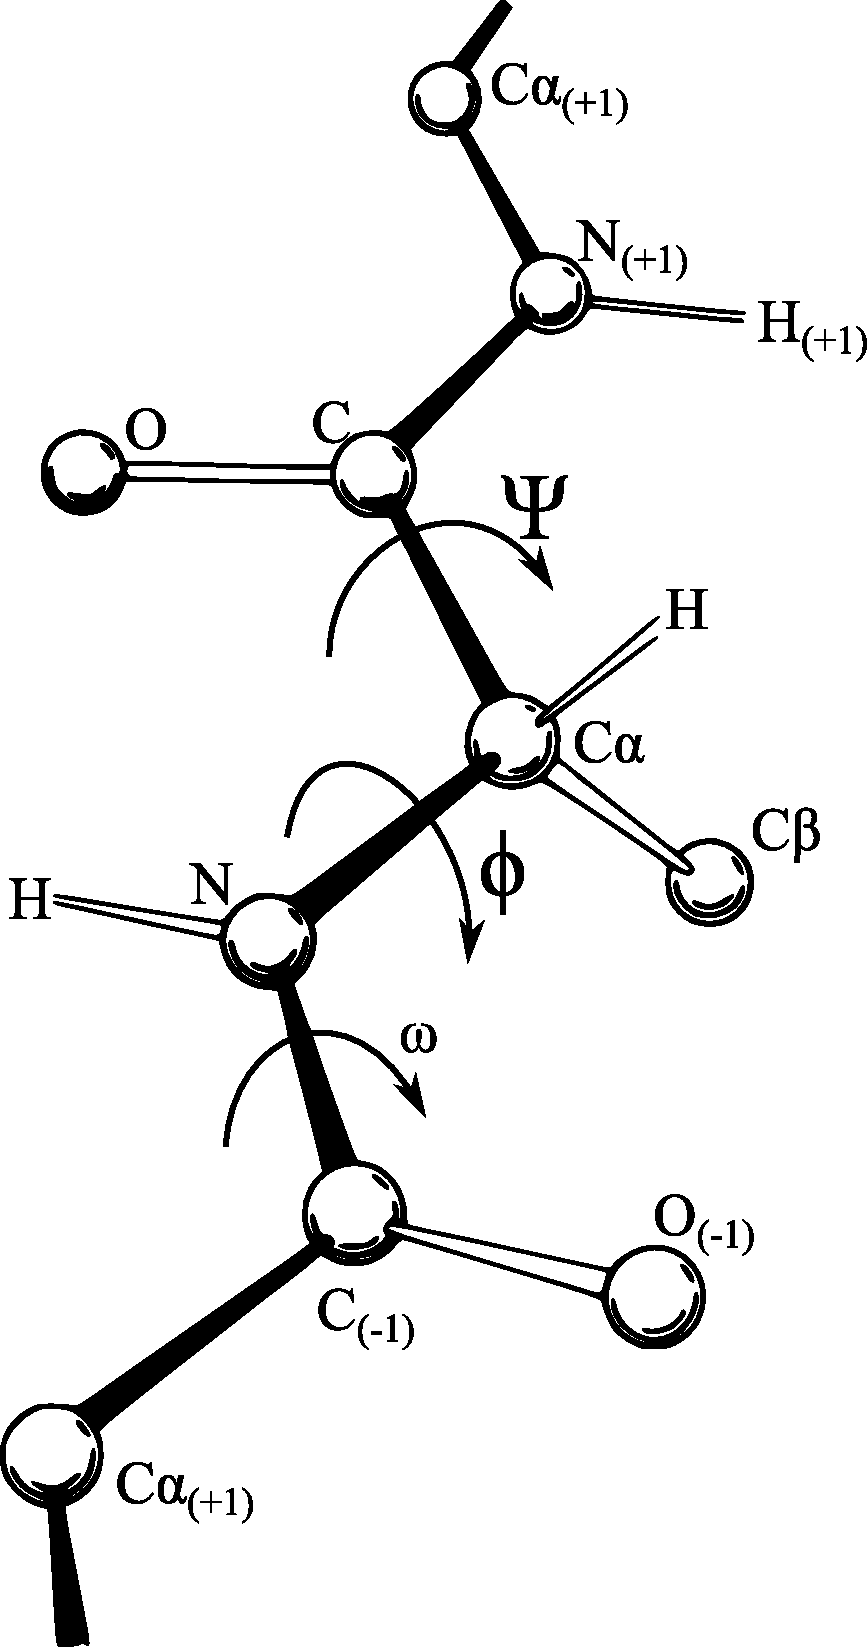
\includegraphics[width=0.30\textwidth]{{images/Protein_backbone_PhiPsiOmega_drawing}.pdf}\\
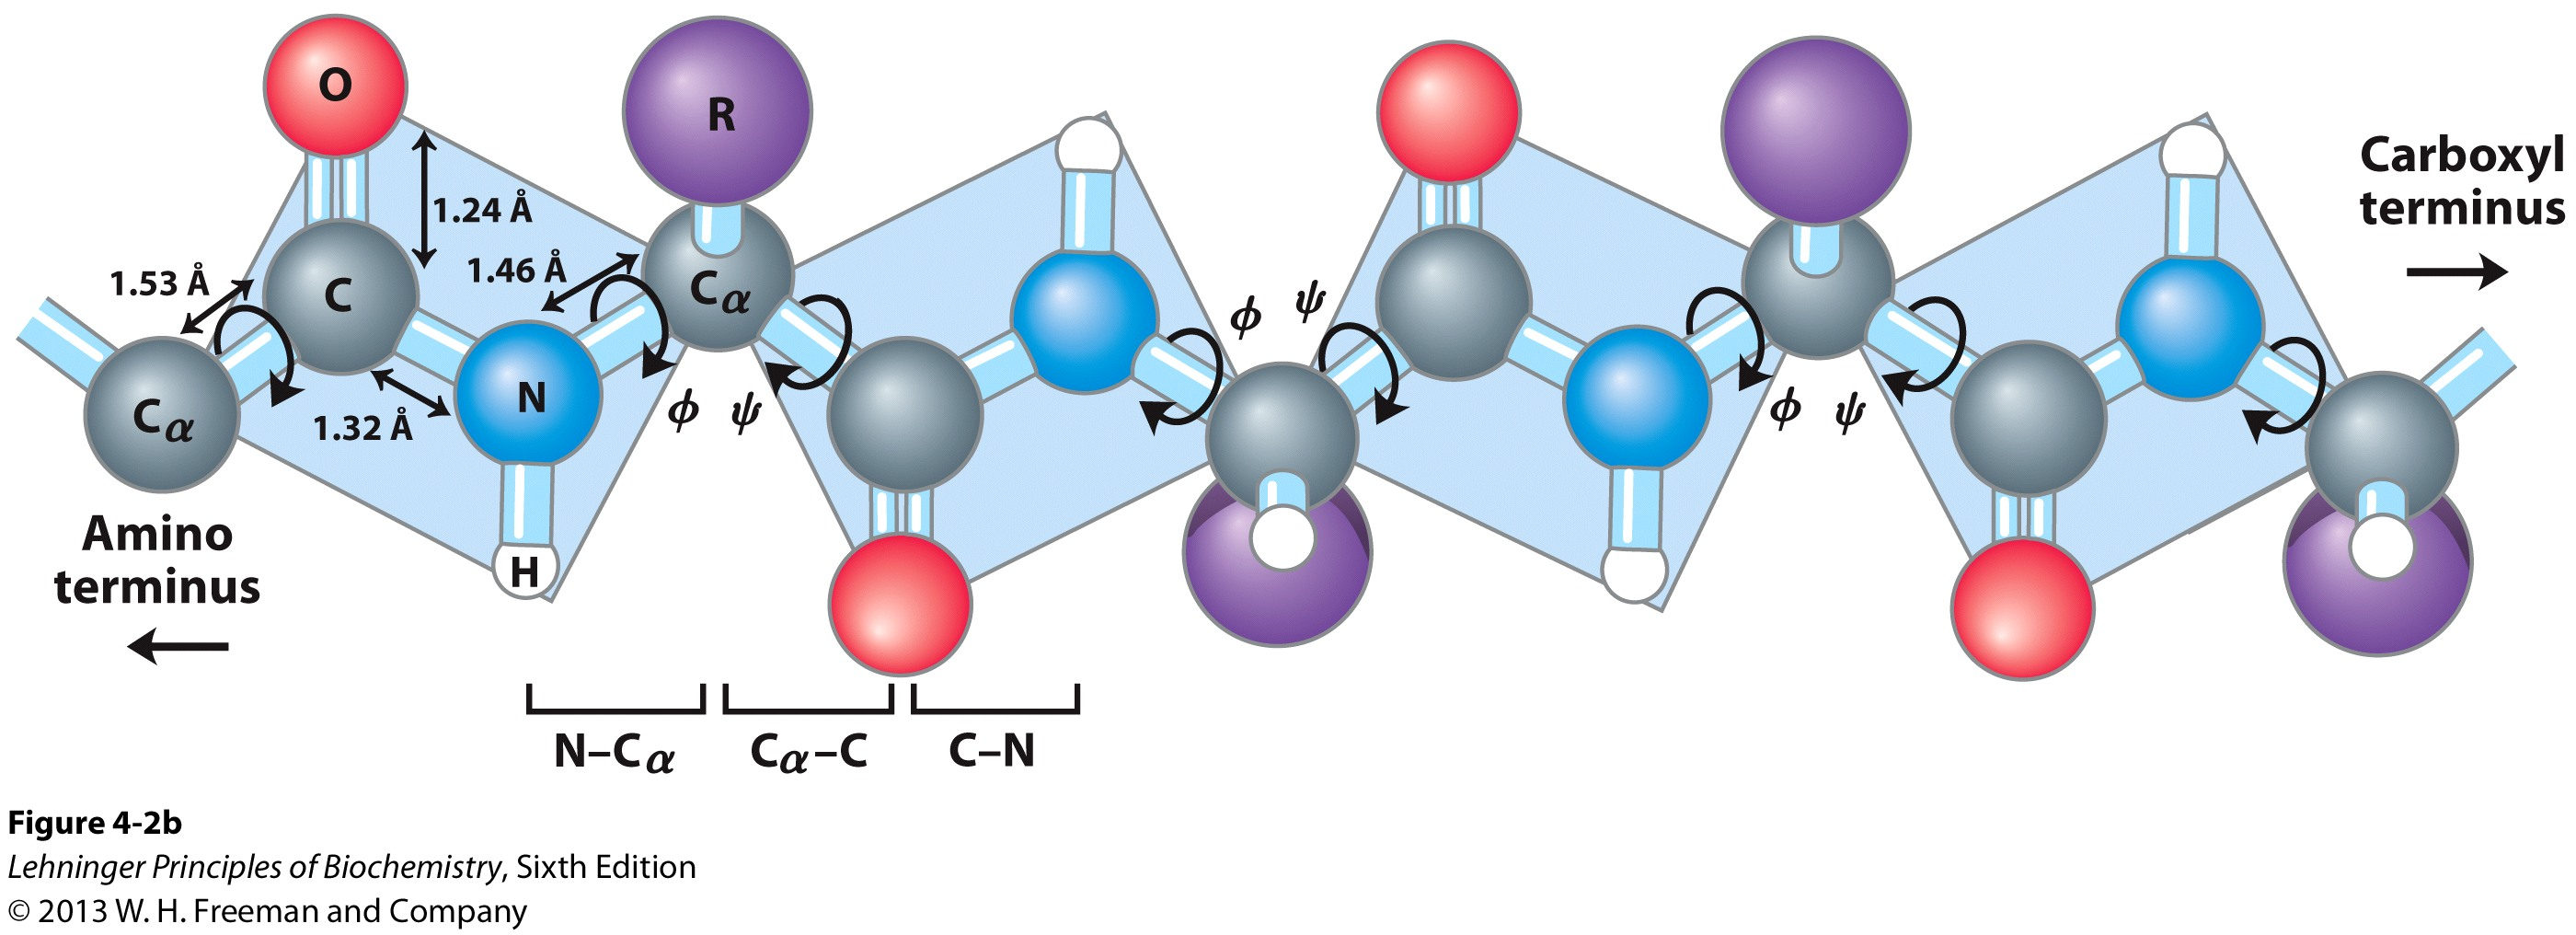
\includegraphics[width=1.0\textwidth]{{images/rama}.jpg}\\
 \caption{Ramachandran angles}
 \label{fig:ramachandranangles}
 \end{figure}

When  finished save the refine penton as \iii{emd\_\humanAdenoMap\_penton\_fitted\_validated.pdb}.
 
Exercise: Go to those regions with worst validation and fix them.

\subsection{Coot: tracing de novo}
\marginnote{\hl{This is difficult!}}[1cm]
We did a secondary structure prediction and save the results in \iii{secondary\_prediction.pdf}. Check if the prediction was reliable. In particular, identify in the prediction the three largest $\alpha$-helices and check in coot if they exists in the traced chain.

Now image that we do not have a homologue to start with and trace the alpha helix.
\begin{itemize}
 \item There should be an $\alpha$-helix starting in aminoacid 174, go there
 \item place a new $\alpha$-helix. \ttt{calculate} $\rightarrow$ \ttt{other modeling tools} $\rightarrow$ \ttt{place helix here}
 \item an alanine $\alpha$-helix appears, you may mutate it with \ttt{calculate} $\rightarrow$ \ttt{align and mutate} or clicking the  \ttt{simple mutate} icon.
\end{itemize}


\section{Molprobity}
MolProbity is a structure-validation web service. A typical MolProbity session starts with the user uploading a coordinate file of their own or fetching one from the PDB, H atoms are added and finally different constraints are verified. The system provides a number that summarizes up to which point the chemical constrains are satisfied. Molprobity is available at: \url{http://molprobity.biochem.duke.edu/}
\marginnote{\hl{URL}}[0cm]
\marginnote{\hl{matchmaker}}[1cm]

Exercise-0: if not done yet check saccharomyces cerevisiae triosephosphate isomerase with 3ypi (2.8\AA-1991), 1ypi(1.9\AA-1990) and 1ney(1.2\AA-2003).

Exercise-1: Execute MolProbity with the penton extracted from the human adenovirus: PDBID=3iyn (you will need to remove unwanted chains first \ttt{chimera} \ra \ttt{model panel} \ra \iii{select chain} \ra \ttt{close} \ra \ttt{write}).

Exercise-2: Execute MolProbity with the refined penton ( \iii{emd\_\humanAdenoMap\_penton\_fitted\_validated.pdb}).

\section{Clashes and Contacts}
Finally, let us check if there are clashes/contacts in your refined macromolecule  \iii{emd\_\humanAdenoMap\_penton\_fitted\_validated.pdb}. After refining the macromolecule with refmac the atomic positions has been modified so there are no clashes. At this point may be interesting to check if there are contacts (bonds) between different aminoacids. Execute \ttt{chimera emd\_\humanAdenoMap\_penton\_fitted\_validated.pdb}. Then, \ttt{Select} \ra {Select all} \ra  \ttt{tools} \ra \ttt{Structure Analysis} \ra \ttt{Find Clashes/contacts}\ra \ttt{Include intramolecule contacts} \ra \ttt{designate} \ra \ttt{themselves} \ra \ttt{contact} \ra \ttt{Apply}.

Usually the inter molecule information is not very interesting and only interaction between different 
molecules are reported. Repeat the experiment but first check that the \ttt{chimera emd\_\humanAdenoMap\_penton\_fitted\_validated.pdb} has symmetry information (that is lines starting with REMARK 350 ...). If it is not there copy it from \iii{first\_guess\_p.pdb}. After adding the symmetry information load the file in \ttt{chimera} and apply the symmetry \ttt{sym \#0}. In \ttt{model panel} close all copies except the five that form a single penton and then compute again clashes and contacts:
\ttt{Select} \ra {Select chain} \ra  \ttt{A} \ra \ttt{tools} \ra \ttt{Structure Analysis} \ra \ttt{Find Clashes/contacts}  \ra \ttt{all other atoms}\ra \ttt{designate} \ra \ttt{contact} \ra \ttt{Apply}.


Example of overlap file:
\begin{verbatim}
Allowed overlap: -0.4
H-bond overlap reduction: 0
Ignore contacts between atoms separated by 4 bonds or less
Detect intra-residue contacts: False
Detect intra-molecule contacts: False

129 contacts
atom1  atom2  overlap  distance
#0 ASN 332.M ND2  #3 ASN 527.B ND2  0.425  2.855
#0 ASN 46.M ND2   #3 ARG 637.B CB   0.388  3.132
#0 ILE 49.M CD1   #3 PRO 644.B CD   0.368  3.392
#0 GLU 45.M OE1   #3 ARG 637.B NH2  0.351  2.709
#0 VAL 66.M CG2   #3 ARG 617.B NH1  0.320  3.200

\end{verbatim}

If the sphere surfaces are 1\AA apart, the  overlap is -1. The overlap between two atoms is defined as the sum of their VDW radii minus the distance between them and minus an allowance for potentially hydrogen-bonded pairs (see \url{http://www.cgl.ucsf.edu/chimera/docs/ContributedSoftware/findclash/findclash.html})

For detecting clashes, cutoff values of 0.4-1.0\AA and allowance values of 0.2-0.6\AA are generally reasonable (default clash criteria 0.6 and 0.4\AA, respectively).

For detecting contacts, negative cutoff values of 0.0-(–1.0)\AA with an allowance of 0.0\AA are generally reasonable (default contact criteria –0.4 and 0.0 Å, respectively).


\newpage
\appendix 
\section {CCP4 header}
\label{app:ccp4header}
\begin{verbatim}
The MRC file format used by IMOD.

The MRC header, length 1024 bytes.  Names are the names used in C code.

OFFSET  NAME            Description

 1      NC              # of Columns    (fastest changing in map)
 2      NR              # of Rows
 3      NS              # of Sections   (slowest changing in map)
 4      MODE            Data type
                          0 = envelope stored as signed bytes (from
                              -128 lowest to 127 highest)
                          1 = Image     stored as Integer*2
                          2 = Image     stored as Reals
                          3 = Transform stored as Complex Integer*2
                          4 = Transform stored as Complex Reals
                          5 == 0	
 
                          Note: Mode 2 is the normal mode used in
                                the CCP4 programs. Other modes than 2 and 0
                                may NOT WORK
 
 5      NCSTART         Number of first COLUMN  in map
 6      NRSTART         Number of first ROW     in map
 7      NSSTART         Number of first SECTION in map
 8      NX              Number of intervals along X
 9      NY              Number of intervals along Y
10      NZ              Number of intervals along Z
11      X length        Cell Dimensions (Angstroms)
12      Y length                     "
13      Z length                     "
14      Alpha           Cell Angles     (Degrees)
15      Beta                         "
16      Gamma                        "\end{verbatim}

% Have a good night. 
% 
% %\bibliographystyle{apalike}
% %\bibliography{tutorial_common/em}


\section {Program: changeheader.py}
\label{app:changeheader}
\lstset{language=Python,caption={changeheader.py: edit MRC files},
        basicstyle=\footnotesize, showstringspaces=false}

\begin{lstlisting}
import struct
import collections
import sys
import os


def saveFile(filename,chain, dataDictionary):
   "overwrite header without overwriting the file"""
   ss=struct.Struct(chain)
   t=tuple(dataDictionary.values())
   packed_data = ss.pack(*t)
   f = open(filename, 'r+')
   f.write(packed_data)
   f.close()

def printDic(dictionary):
    print "-------------------------"
    for key, value in header.iteritems() :
       print key, value
    print "-------------------------"

#process command line
if len(sys.argv) < 2:
   print "Usage: %s 3DmapFileName"%sys.argv[0]
   exit(1)
else:
   filename = sys.argv[1]

f = open(filename,'rb')
s = f.read(13*4)#read header up to angles
f.close()
chain = "< 3i i 3i 3i 3f"
header = collections.OrderedDict()
a = struct.unpack(chain, s)
#header['Dim-------------']=""
header['NC'] = a[0]
header['NR'] = a[1]
header['NS'] = a[2]
header['Mode (should be 2)'] = a[3]
#header['VOXEL (0,0,0) is at coordinate (in pixels)-------------']=""
header['NCSTART'] = a[4]
header['NRSTART'] = a[5]
header['NSSTART'] = a[6]
#header['Number of intervals along...-----------------']=""
header['NX'] = a[7]
header['NY'] = a[8]
header['NZ'] = a[9]
#header['Cell Dimensions (Angstroms) -usually wrong-------------']=""
header['X-length'] = a[10]
header['Y-length'] = a[11]
header['Z-length'] = a[12]
#header['sampling rate (Z)'] = a[12]/a[9]

headerDouble=['X-length','Y-length','Z-length']

printDic(header)

print """\nType label=value<enter> (NX=4, do not introduce spaces), 
s<enter> to save the file or 
press q<enter> for quiting
\n""" 
line = sys.stdin.readline()
while line:
    words = line.rstrip().split("=")
    key = words[0]
    if key=="q":
         break
    elif key=="s":
         print("save file %s"%filename)
         saveFile(filename, chain, header)
         break
    if key in header:
        value = words[1]
        if key in headerDouble:
            header[key]=float(value) # double
        else:
            header[key]=int(value) # int
    else:
        print "unknow key %s"%words[0]
    printDic(header)
    line = sys.stdin.readline()
\end{lstlisting}
\end{document}
